% Relatório do TCC2: edição mantida diretamente neste arquivo LaTeX.
\chapter{Inspirações visuais e de jogabilidade}\label{cap:tcc2-3}

\textit{Quake III Arena} e \textit{Unreal Tournament} inspiraram o combate em arena, a coleta de recursos e a disputa por objetivos. No jogo desenvolvido, essas ideias aparecem nas armas, nos itens coletáveis e nos modos Team Deathmatch e King of the Hill. \cite{QUAKE} \cite{UNREAL}

\textit{Lovely Planet} serviu de referência para a combinação de tiros com saltos e para uma apresentação visual colorida e simplificada, ilustrada na Figura~\ref{fig:inspiracao-lovely-planet}. O projeto incorporou salto duplo e plataformas de impulso, além de usar cores para identificar os times. \cite{LOVELY}

\begin{figure}[htbp]
\centering
\caption{Referência visual do jogo \textit{Lovely Planet}}
\label{fig:inspiracao-lovely-planet}
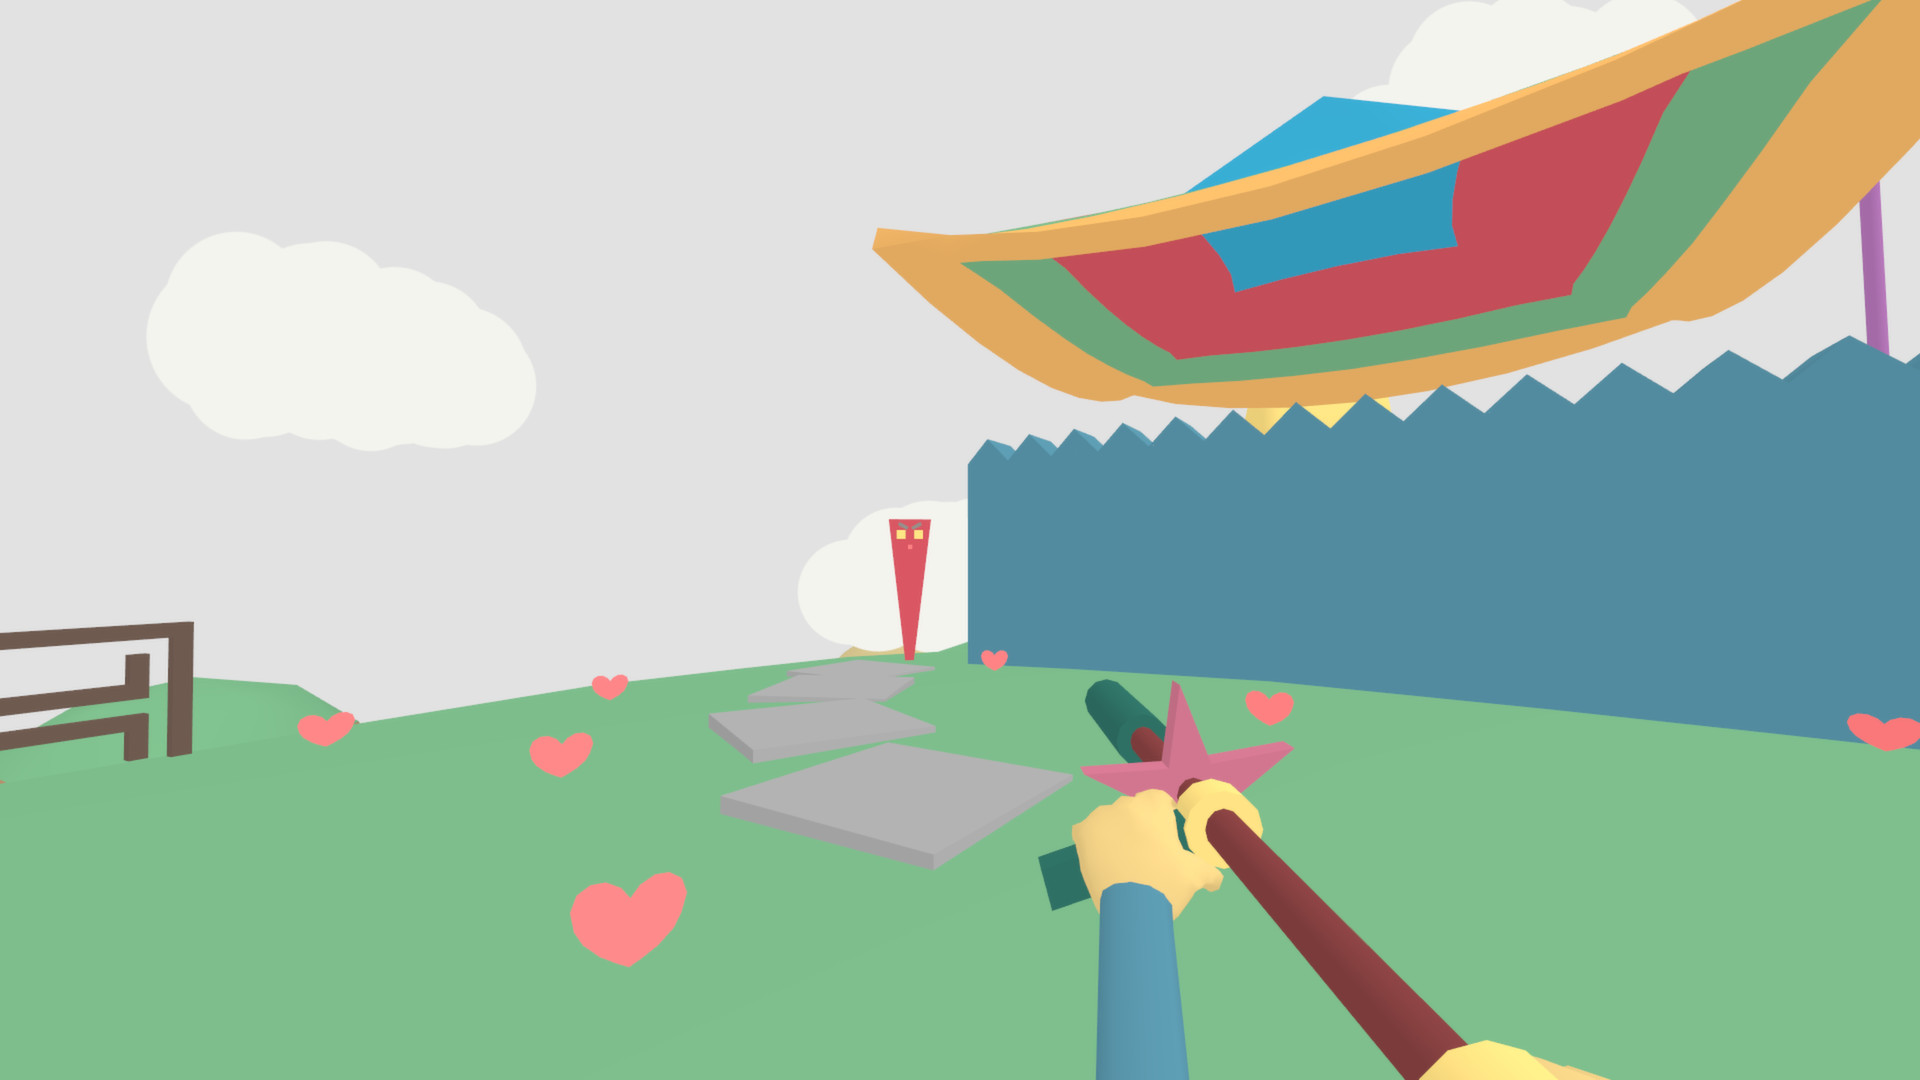
\includegraphics[width=0.88\linewidth]{imgs/lovelyplanet.jpg}
\fonte{imagem de \textit{Lovely Planet} utilizada no TCC1 \cite{LOVELY}}
\end{figure}
